\documentclass[12pt,preprint]{aastex}


\usepackage{graphicx}
\graphicspath{{./}}


%%%%%%%%%%%%%%%%%%%%%%%%%%%%%%%%%%%%%%%%%%%%%%%%%%%%
%%% author-defined commands
\newcommand\about     {\hbox{$\sim$}}
\newcommand\x         {\hbox{$\times$}}
\newcommand\othername {\hbox{$\dots$}}
\def\eq#1{\begin{equation} #1 \end{equation}}
\def\eqarray#1{\begin{eqnarray} #1 \end{eqnarray}}
\def\eqarraylet#1{\begin{mathletters}\begin{eqnarray} #1 %
                  \end{eqnarray}\end{mathletters}}
\def\non    {\nonumber \\}
\def\DS     {\displaystyle}
\def\E#1{\hbox{$10^{#1}$}}
\def\sub#1{_{\rm #1}}
\def\case#1/#2{\hbox{$\frac{#1}{#2}$}}
\def\about  {\hbox{$\sim$}}
\def\x      {\hbox{$\times$}}
\def\ug               {\hbox{$u-g$}}
\def\gr               {\hbox{$g-r$}}
\def\ri               {\hbox{$r-i$}}
\def\iz               {\hbox{$i-z$}}
\def\a                {\hbox{$a^*$}}
\def\O                {\hbox{$O$}}
\def\E                {\hbox{$E$}}
\def\Oa               {\hbox{$O_a$}}
\def\Ea               {\hbox{$E_a$}}
\def\Jg               {\hbox{$J_g$}}
\def\Fg               {\hbox{$F_g$}}
\def\J                {\hbox{$J$}}
\def\F                {\hbox{$F$}}
\def\N                {\hbox{$N$}}
\def\dd               {\hbox{deg/day}}
\def\mic              {\hbox{$\mu{\rm m}$}}
\def\Mo{\hbox{$M_{\odot}$}}
\def\Lo{\hbox{$L_{\odot}$}}
\def\comm#1           {\tt #1}
\def\refto#1          {\ref #1}
\def\T#1              {({\bf #1})}
\def\H#1              {({\it #1})}

%%%%%%%%%%%%%%%%%%%%%%%%%%%%%%%%%%%%%%%%%%%%%%%%%%%%

\begin{document}


\title{ {\bf Term Project \# 3}}  
                   
Galactic Astronomy (Astr 511); Winter Quarter 2015

prof. \v{Z}eljko Ivezi\'{c}, University of Washington


\section{Introduction} 

We will boldly attempt heroic collaborative work: two awesome teams working on
cutting-edge problems using recently released APOGEE-ASPCAP 
data\footnote{See http://www.sdss.org/dr12/irspec/}:
\begin{itemize} 
\item {\bf EXD:} using abundances for 15 elements (from summary allStar file), we will study the 
variation of their 15-D abdundance distribution in the 3-dimensional $XYZ$ space, as a function 
of stellar population (halo, thin disk, thick disk); we will use Extreme Deconvolution (EXD) method to 
quantify the 15-D distributions, see astroML Book Figures 6.11 and 6.12; nevertheless, it may be
prudent to run PCA on the set of these 15-D vectors before attempting (more complicated) EXD (see
below). 
\item {\bf DimRed:} Using spectra (apStar files, one per star), we will run dimensionality-reduction
methods PCA, ICA and NMF and analysis results; see astroML Book Figures 7.4, 7.6 and 7.7. 
\end{itemize}    

The basic ``building blocks'' are same for both projects: 
\begin{enumerate}
\item define the teams, and within each team assign responsibilities for the tasks below; 
\item learning about the data properties and starting a paper/notes with a brief Introduction 
about APOGEE and data properties;  paper templates can be copied from the class 
repo\footnote{Astr511/tree/master/HW2015/Project3} to  appropriate directory within the 
new 2015ASTR511 repo. 
\item learning about how to download and access data (including writing python code);  
\item learning about how to (modify and) run appropriate astroML tools; 
\item writing analysis summary (including plots) for the paper 
\end{enumerate}



\section{Project EXD}

Copying verbatim from the SDSS Data Release webpage\footnote{http://www.sdss.org/dr12/irspec/aspcap/},
``The APOGEE Stellar Parameters and Chemical Abundances Pipeline (ASPCAP) employs a two-step process 
to extract abundances: first, determination of the atmospheric parameters by fitting the entire APOGEE spectrum, 
and second, use of these parameters to fit various small regions of the spectrum dominated by spectral features
 associated with a particular element in order to derive the individual element abundance.''
The first step of ASPCAP estimates seven parameters: effective temperature, surface gravity, microturbulence, 
overall metal abundance $[M/H]$, relative $\alpha$-element abundance $[\alpha/M]$ (defined as O, Mg, Si, S, 
Ca, and Ti changing with solar proportions in lockstep), carbon $[C/M]$, and nitrogen $[N/M]$ abundances.
The second step estimates abundances of the following 15 elements: Al, Ca, C, Fe, K, Mg, Mn, Na, Ni, N, O, Si, S, Ti, and V.

These stellar parameters and abundances (for 163,278 stars) are conveniently stored in a single fits file; the 
current version (Data Release 12) is allStar-v603.fits. I played a bit with this file and added my sample analysis 
code (plain .py files -- not ipython notebooks!), in files allStarAnalysis1.py and allStarAnalysis2.py, to repo 
2015ASTR511/Project3. If you download these files and allStar-v603.fits data file, you will be able to reproduce
figures 1 and 2 here. 

This initial analysis is not very deep, and is missing a proper flag selection (I did some ad hoc shortcuts).
The plots don't show it, but I was happy when I managed to reproduce a good agreement between 
the $[\alpha/Fe]$ value estimated during the first ASPCAP stage, and a corresponding value based on the
measured abundances of individual $\alpha$ elements. If the data are read as 
\begin{verbatim}
data = pyfits.open('allStar-v603.fits')[1].data[::1] 
\end{verbatim}
then $[\alpha/Fe]$ from the first stage can be accessed as 
\begin{verbatim}
alphaFe = data['PARAM_ALPHA_M']
\end{verbatim}
while individual abundances can be accessed as, e.g. for Mg and Ti,
\begin{verbatim}
MgH = data['MG_H']
TiH = data['TI_H']
\end{verbatim}


The $[\alpha/Fe]$ based on individual abundances can be evaluated as (note that $\alpha$ elements
Ne and Ar are missing): 
\begin{equation}
       [\alpha/Fe]^\ast= {[O/H]+[Mg/H]+[Si/H]+[S/H]+[Ca/H]+[Ti/H] \over 6} - [Fe/H].
\end{equation}
In other words, $[\alpha/Fe]$ corresponds to the {\it mean} value of the abundances of the above six elements, 
and the last term transforms the scale from ``per $H$'' to ``per $Fe$''. 

The difference of the two estimates of $[\alpha/Fe]$ has a median of $-0.008$ dex and rms of 0.042 dex, 
which represents excellent agreement! I also compared the values of $[M/H]$, 
\begin{verbatim}
MH = data['PARAM_M_H']
\end{verbatim}
and $[Fe/H]$, 
\begin{verbatim}
FeH = data['Fe_H']
\end{verbatim}
and their difference has a median of $0.007$ dex and rms of 0.077 dex, 
which is also excellent.

\subsection{Milestones}

Based on the above analysis, here are specific few milestones: 

\begin{enumerate}
\item Reproduce Figures 1 and 2 here, but use proper flag checking. 
\item Run the PCA on the vector of 15 abundances for the cleaned sample (about 100,000 stars) and
plot the first few eigen components. What do they mean? How much variance is captured by these
components? Plot diagrams constructed with eigen coefficients. Do the same separately for high Galactic latitudes ($|b|>20^\circ$) 
and low latitudes  ($|b|<5^\circ$). Do the same separately for halo, thick and thin disk populations defined
by the cuts based on $[Fe/H]$ and $[\alpha/Fe]$ listed below. Do we see any differences? Can we
recognize halo/thick disk/thin disk stars using diagrams constructed with eigen coefficients for
the full sample? 
\item Based on the PCA analysis, decide whether to run the full EXD.  
\end{enumerate} 


Halo, thick and thin disk populations can be approximately defined (see the bottom right panel
in Figure 1) as:
\begin{verbatim}
# define thin/thick/halo subsamples
condHalo = (data['PARAM_M_H'] > -2.5) & (data['PARAM_M_H'] < -1.1))
condDisk = (data['PARAM_M_H'] > -0.9) & (data['PARAM_M_H'] < 0.6))
condThin = (condDisk & (data['PARAM_ALPHA_M'] > 0.0) & (data['PARAM_ALPHA_M'] < 0.15)) 
condThick = (condDisk & (data['PARAM_ALPHA_M'] > 0.15) & (data['PARAM_ALPHA_M'] < 0.35)) 
\end{verbatim}




\section{Project DimRed} 

APOGEE spectra are stored one per star in apStar files\footnote{See http://www.sdss.org/dr12/irspec/spectra/}. 
The combined (from several independent observations, or visits) spectra are generated by resampling individual visits 
onto a common, logarithmically-spaced wavelength scale. The spectra are corrected for each visit’s derived radial 
velocity: {\it the resulting spectra are in rest, vacuum wavelengths!}. Also, these spectra include the barycentric 
correction (the Earth's motion is corrected for). 

The primary HDU of each file contains an 
image which gives the two versions of the combined spectrum for each object, as well as the individual visit 
spectra that went into these combinations. The two versions of the combined spectrum correspond to different 
weighting schemes (using the square of the signal-to-noise ratio): global weighting and pixel-by-pixel weighting.
We will want to work with the version based on pixel-by-pixel weighting. The combined spectra include the
continuum (determined using a 500-pixel median filter, with bad pixels masked).

I have not yet played with apStar files. I would suggest to first download and plot a dozen or so spectra 
to learn technical details before we attempt massive processing. In particular, we will need to understand how
to treat pixel masks (bitmasks). 

Generally speaking, we will want to process various subsets of the full set. Hence, when writing code 
to feed tools from astroML with these spectra, we need to develope a ``pre-processor'' that will collect
the required spectra and send the selected subset downstream. 


\subsection{Milestones}

Here are a few milestones to start with
\begin{enumerate}
\item Ask the other team for a few examples of stars (say, a dozen each) from halo, thick and thin disk populations.
Plot their spectra. 
\item Run the PCA method on this small set.
\item If everything went fine, download the entire dataset (about 163,278 apStar files) and run the PCA on 
all of them. Beware of flags, missing/masked pixels, etc. 
\item Plot the first few eigen components. What do they mean? How much variance is captured by these
components?
\item Plot diagrams constructed with eigen coefficients. Can we
recognize halo/thick disk/thin disk stars (classified using cuts based on $[Fe/H]$ and $[\alpha/Fe]$, see
other project) using diagrams constructed with eigen coefficients? That is, color-code points according 
to population (or use contours of different colors). 
\item Based on the PCA analysis, decide whether to run the ICA and NMF analysis. 
\end{enumerate} 


\begin{figure}
  \centering
  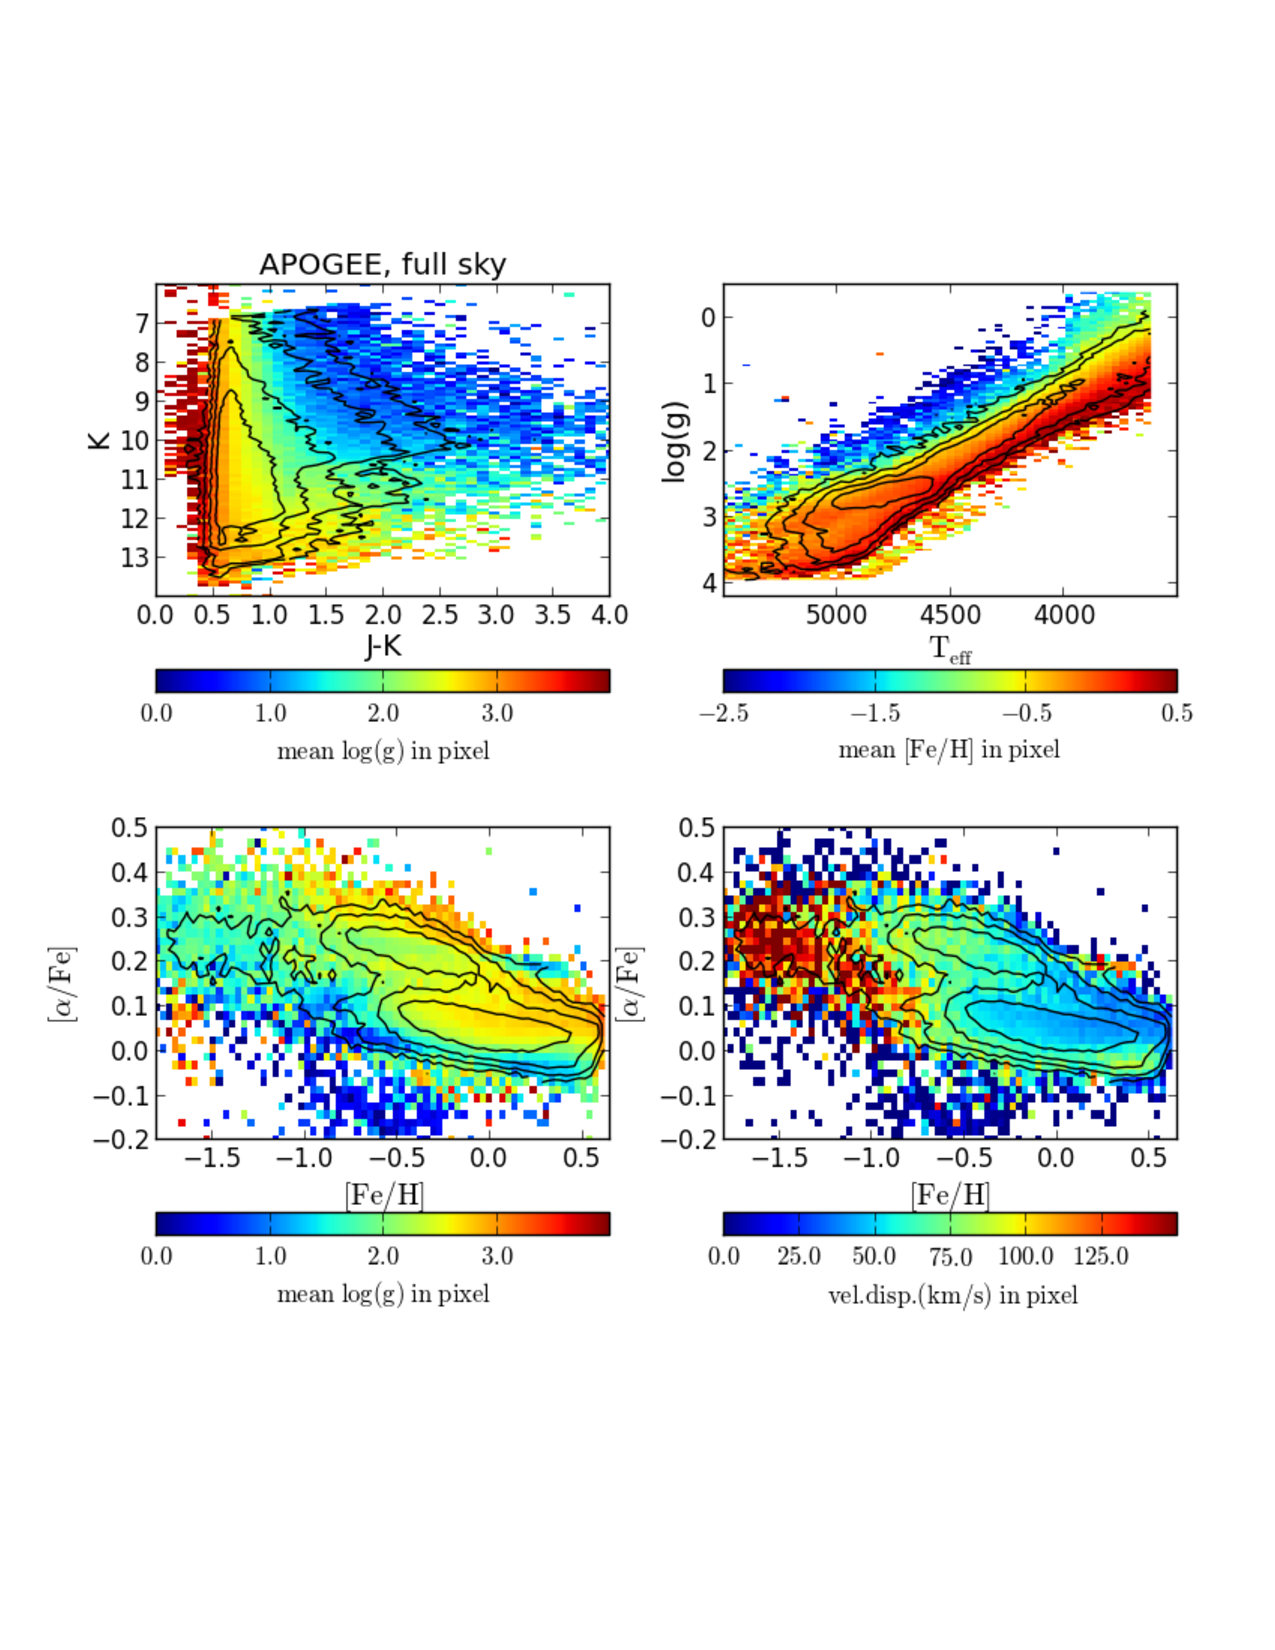
\includegraphics[width=\textwidth]{apogee1.pdf}
  \vskip -1.5in
  \caption{
    This figure was produced with allStarAnalysis1.py. It shows various two-dimensional diagrams  
    for a subset of stars from allStar-v603.fits data file, color-coded using a third quantity marked
    below each panel. 
  }
  \label{basic_example1}
\end{figure}


\begin{figure}
  \centering
  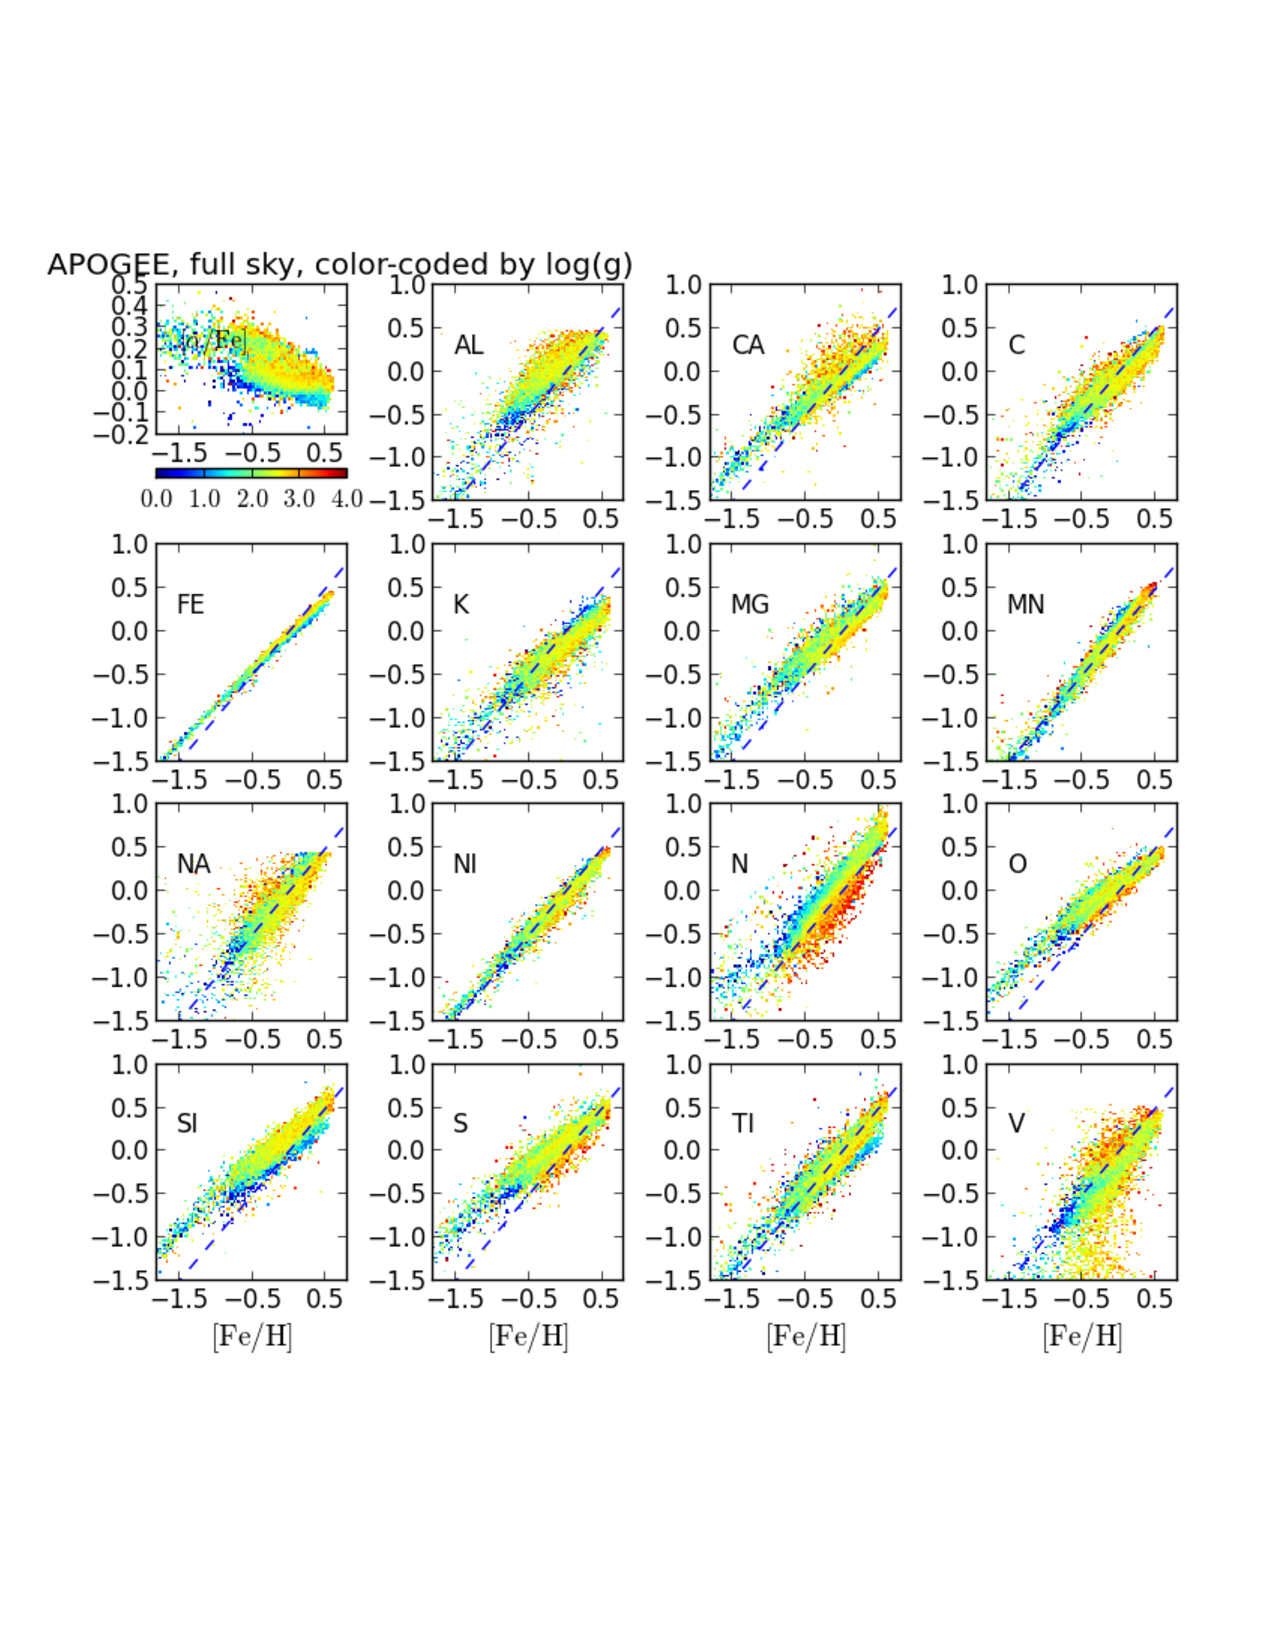
\includegraphics[width=\textwidth]{apogee2.pdf}
  \vskip -1.5in
  \caption{
    This figure was produced with allStarAnalysis2.py. The top left panel shows the $[\alpha/Fe]$ vs. 
$[Fe/H]$ diagram for a subset of stars from allStar-v603.fits data file, color-coded using $log(g)$. 
The remaining 15 panels show the abundances of 15 individual elements, labeled in each panel, 
vs. $[Fe/H]$, using the same color-coding as in the top left panel. 
  }
  \label{basic_example2}
\end{figure}


\end{document}













The data file Astr511HW3data.dat (linked to class webpage as
a gzipped file) contains SDSS photometric measurements for 
about 900,000 stars from the so-called Stripe 82\footnote{For
details see http://www.astro.washington.edu/users/ivezic/sdss/catalogs/stripe82.html}.
This sky area is defined by $|Dec|<1.267^\circ$ and $-66^\circ < RA < 73^\circ$. 
The catalog includes all sources from Stripe 82 that satisfy
the following criteria:
\begin{enumerate}
\item Unresolved source in imaging data
\item Processing flags BRIGHT, SATUR, BLENDED, or EDGE are not set
\item At least 4 observations in $ugr$ bands
\item Flux limit: $u<22$
\item Color selection of F/G stars: $0.6 < (u-g) <2.2$ and $0.2 < (g-r) < 0.6$ and
      $0 < 0.50(u-g) - (g-r) + 0.05 < 0.5$
\item Non-variable: $\chi^2_{pdf} < 10$ in the $g$ band
\end{enumerate}

The data are listed as one line per star, with each line containing 
the following quantities:
\begin{itemize}
\item {\bf ra dec:} right ascension and declination (J2000.0)
 in decimal degrees 
\item {\bf Ar:} the value of the $r$ band ISM extinction used to 
     correct photometry (adopted from the SFD maps; for bands 
     other than $r$, standard SDSS coefficients are used)
\item {\bf u g r i z:} SDSS photometry (already corrected for the ISM
       extinction)
\item {\bf uErr gErr rErr iErr zErr:} photometric errors
\end{itemize}

For stars from this file, compute absolute magnitude and distance
using a photometric parallax relation, $M_r(g-i,[Fe/H])$, given
by eqs. A2, A3 and A7 from
 Ivezi\'{c} et al. 2008 (ApJ, 684, 287).
For computing metallicity, $[Fe/H]$, instead of their
eq.~4, use an updated expression from Bond et al. 2010 (ApJ, 716, 1): 


\begin{equation}
\label{Zphotom}
  [Fe/H] = A + Bx + Cy + Dxy  + Ex^2 + Fy^2 + Gx^2 y + Hxy^2 + Ix^3 + Jy^3,
\end{equation}
with $x=(u-g)$ and $y=(g-r)$, and the best-fit coefficients ($A$--$J$) = 
($-$13.13, 14.09, 28.04, $-$5.51, $-$5.90, $-$58.68, 9.14, $-$20.61, 0.0,
58.20). Yes, these are the same expressions as in Homework 1, and you
can (and should) recycle your code.

Given the position and distance, we can now make various 
metallicity maps. Because this is coadded data, it extends
about a factor of two further in distance than the sample
analyzed in Ivezi\'{c} et al. (2008).

Split the sample into four subsamples using 0.1 mag wide bins
of $g-r$ color (from 0.2 to 0.6). For each subsample make the 
following polar plots\footnote{$X$ and $Y$ have nothing to do with 
Galactic $X$ and $Y$ coordinates seen in some figures from the 
lectures; $X$ and $Y$ here are simply convenient projection coordinates 
for stripe 82 geometry.} 
($X=D\sin(RA)$, $Y=D\cos(RA)$; also, 
in all plots draw lines of constant galactocentric cylindrical 
radius of 10, 15 and 20 kpc, and constant distance from the 
galactic plane, $|Z|$, of 5, 10 and 15 kpc):
\begin{enumerate}
\item Plot the $\ln(N/D)$ map, where $N$ is the number of stars
  in a given $X-Y$ bin (pixel), and $D$ is the median distance to all 
  stars in that pixel.
  This quantity is proportional to the local stellar number density
  (because the ``third'' coordinate is defined by the SDSS scan width 
   of $\sim$2.5$^\circ$). 
  Is it consistent with the model from Juri\'{c} et al. (2008, ApJ, 673, 864)?
  Are there unexpected features, suspected data artefacts, etc? 
\item Plot the median $[Fe/H]$ map. Is it consistent with the model from 
 Ivezi\'{c} et al. (2008, ApJ, 684, 287)? Are there unexpected features, 
 suspected data artefacts, etc?   
\item Plot the map for $[Fe/H]$ root-mean-square (rms) scatter per pixel.
Is the rms scatter constant? If not, think of an explanation for the observed 
variation.
\item Plot the skewness map for $[Fe/H]$ (the skewness for small samples
is defined in eq.~2 from Sesar et al. 2007, AJ, 134, 2236). Is your
map consistent with a Gaussian distribution of $[Fe/H]$?
\item Think of a method/metric/statistic for finding deviations from
Gaussianity and make a map! Did you find any deviations? Streams, 
bad data, other junk? 
\end{enumerate}


\end{document}










latex tpApogee; dvips -o tpApogee.ps tpApogee; ps2pdf tpApogee.ps 